%----------------------------------------------------------------------------------------
%	PACKAGES AND DOCUMENT CONFIGURATIONS
%----------------------------------------------------------------------------------------
\documentclass[11pt]{article}
\usepackage{amsmath} % Required for some math elements
\usepackage{hyperref} 
\usepackage{xcolor}
\usepackage{lipsum} 
\usepackage{cite}
\usepackage{graphicx} % Required for the inclusion of images
\usepackage{algorithmic}
\usepackage{array}
\usepackage{bookmark}
\usepackage{listings}
\usepackage{amssymb}
\usepackage{enumitem}
\usepackage[margin=16mm]{geometry}
\usepackage[caption=false, font=footnotesize]{subfig}
\usepackage{fancyhdr}
\pagestyle{fancy}
\lhead{ENGR222 Assignment 1 Submission}
\rhead{Daniel Eisen : 300447549}
\cfoot{\thepage}
\renewcommand{\headrulewidth}{0.4pt}
\renewcommand{\footrulewidth}{0.4pt}

\newlist{steps}{enumerate}{1}
\setlist[steps, 1]{label = Step \arabic*:}

\hypersetup{ %color attributes of citation, link, etc.
    colorlinks=true,
    linkcolor=blue,
    filecolor=gray,      
    urlcolor=blue,
    citecolor=blue,
}

\newcommand{\matlab}{\textsc{Matlab }} %very important and totally necessary addition

\newcommand\Item[1][]{%
  \ifx\relax#1\relax  \item \else \item[#1] \fi
  \abovedisplayskip=0pt\abovedisplayshortskip=0pt~\vspace*{-\baselineskip}}
%----------------------------------------------------------------------------------------
%	DOCUMENT INFORMATION
%----------------------------------------------------------------------------------------

\title{ENGR 222 \\ Assignment 1 Submission}
\author{Daniel Eisen : 300447549}
\date{\today}

\begin{document}
\maketitle
%----------------------------------------------------------------------------------------
%	DOCUMENT CONTENT
%----------------------------------------------------------------------------------------
\begin{enumerate}
    \item Consider the parametric equations:
          $(f(t),g(t)) = (8sin(t),2t-sin(2t))$
          \begin{enumerate}
              \Item %a
              \begin{align*}
                  (f(t),g(t)) = [ & (0,0),(5.657,0.571),(8,\pi),(5.657,5.712),(0,2\pi), \\
                                  & (-5.657,6.854),(-8,3\pi),(-5.657,11.996),(0,4\pi)]
              \end{align*}

              \begin{center}
                  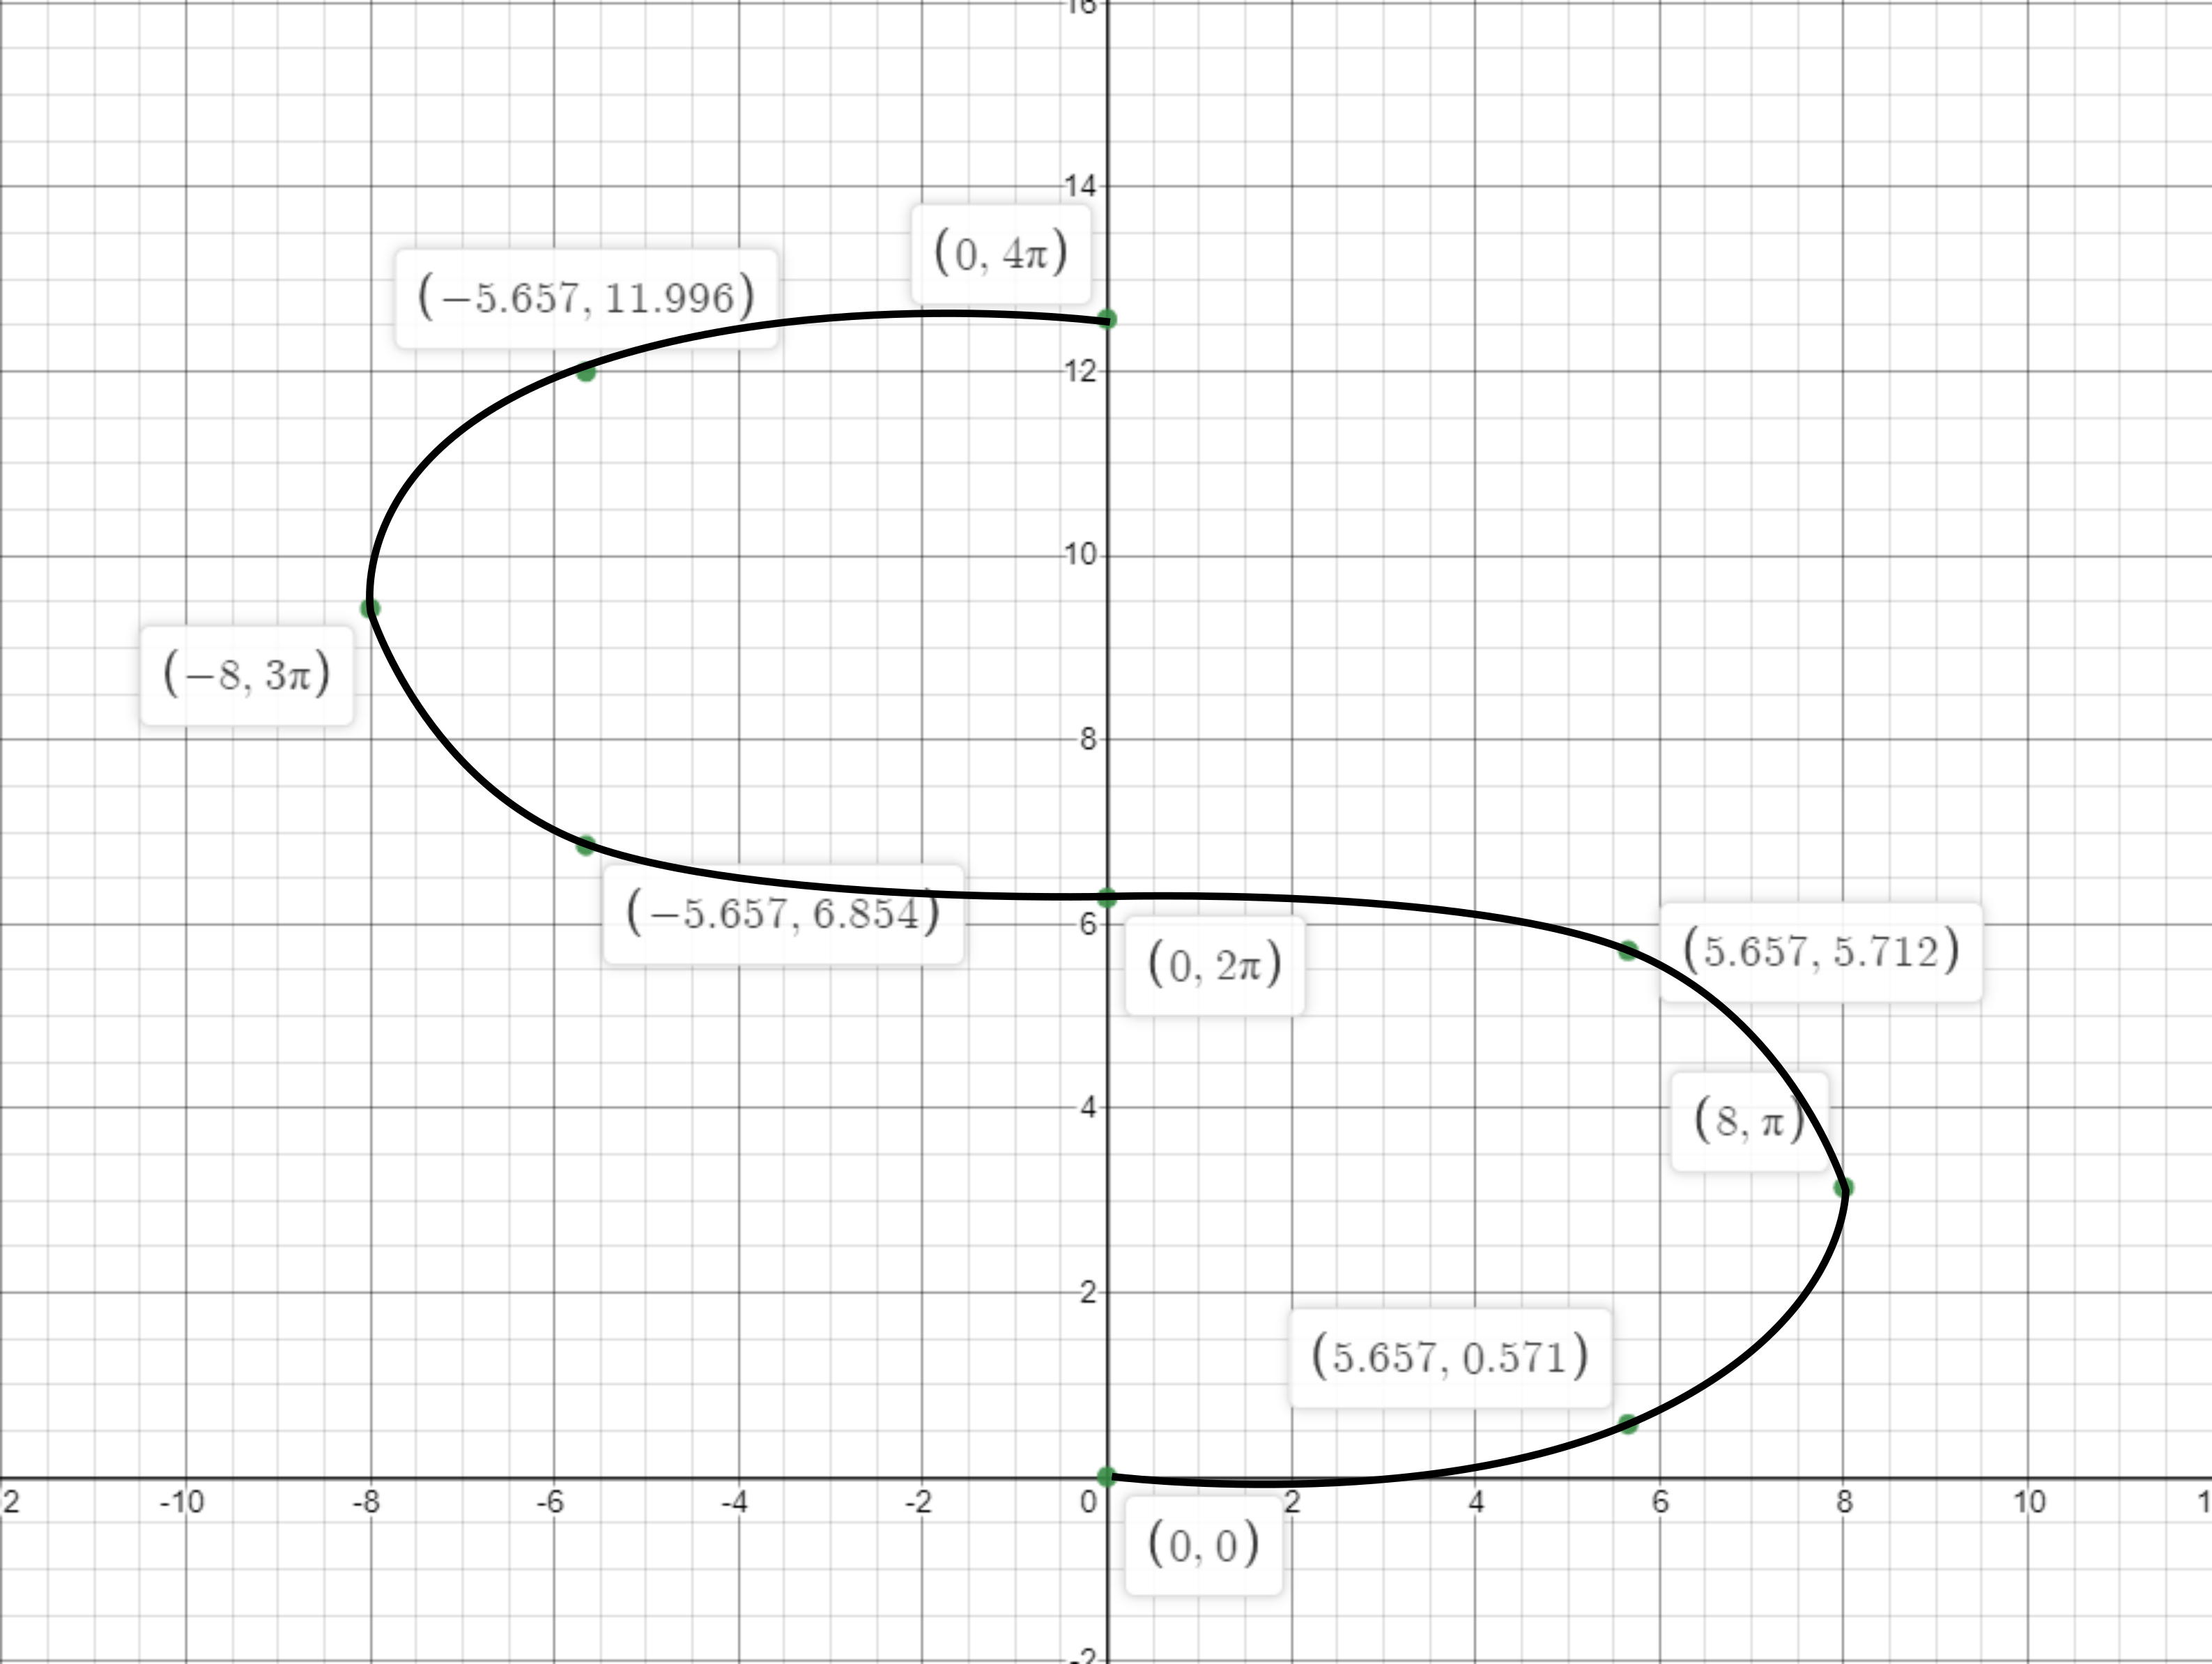
\includegraphics[width=0.4\textwidth]{inc/1a.png}
              \end{center}

              \Item %b
              Tangent vector:\\
              \begin{align*}
                  (f'(t),\; g'(t))               & = (8cos(t), 2 - 2cos(2t)) \\
                  t=\pi/6 \;:\; (f'(t),\; g'(t)) & = (6.928203,1)            \\
              \end{align*}
              Unit tangent vector:\\
              \begin{align*}
                  \frac{(f'(t),\; g'(t))}{\| (f'(t),\; g'(t)) \|} = \frac{(6.928203,1)}{\sqrt{6.928203^2+1}} = \left(\frac{6.928203}{7},\frac{1}{7}\right)
              \end{align*}

              \Item %c
              Tangent Line equation (normalised):\\
              \begin{align*}
                   & = (x,y) + t{\cdot} \frac{(f'(t),\; g'(t))}{\| (f'(t),\; g'(t)) \|} \\
                   & = (4,0.181) + t\left(\frac{6.928203}{7},\frac{1}{7}\right)         \\
                   & = \left(\frac{6.928203t}{7}+4,\frac{t}{7}+0.181)\right)
              \end{align*}

              \Item %d
              Normal line:
              \begin{align*}
                   & = \left( f(\frac{\pi}{6}) - tg'(\frac{\pi}{6}), g(\frac{\pi}{6}) + tf'(\frac{\pi}{6}) \right) \\
                   & = \left( 4 - t, 0.181 + 6.928203t \right)
              \end{align*}

              \Item %e
              Arc length:
              \begin{align*}
                  L & = \int_{0}^{2\pi}\sqrt{f'\left(t\right)^{2}+g'\left(t\right)^{2}}dt                                                          \\
                    & = \int_{0}^{2\pi}\sqrt{\left(8\cos\left(t\right)\right)^{2}+\left(2-2\cos\left(2t\right)\right)^{2}}dt                       \\
                    & = \int_{0}^{2\pi}\sqrt{\left(32\cos\left(2t\right)+32\right)+\left(4+4\cos\left(2t\right)^{2}-8\cos\left(2t\right)\right)}dt \\
                    & = \int_{0}^{2\pi}\sqrt{4\cos\left(2t\right)^{2}+24\cos\left(2t\right)+36}dt                                                  \\
                    & = \int_{0}^{2\pi}\sqrt{4\left(\cos\left(2t\right)^{2}+6\cos\left(2t\right)+9\right)}dt                                       \\
                    & = \int_{0}^{2\pi}\sqrt{4\left(\cos\left(2t\right)+3\right)^{2}}dt                                                            \\
                    & = 2\int_{0}^{2\pi}\left(\cos\left(2t\right)+3\right)dt                                                                       \\
                    & = sin(2t) + 6t \Big|_0^{2\pi}                                                                                                \\
                    & = (0+12\pi) - (0+0)                                                                                                          \\
                    & = 12\pi \approx 37.6991118431
              \end{align*}

          \end{enumerate}
    \item Consider the curve described by the vector valued function:\\
          $$\textbf{r}(t) = \frac{e^{2t}-2t}{4}\textbf{i} + e^t\textbf{j}$$
          \begin{enumerate}
              \Item
              \begin{align*}
                  \textbf{r}(t){\cdot}\textbf{j} & =2                       \\
                  e^t                            & = 2                      \\
                  t                              & = ln(2) \approx 0.693147 \\
                  \textbf{r}\left(t=ln(2)\right) & = (0.653,2)
              \end{align*}

              \Item
              \begin{align*}
                  \textbf{r}'(t)       & = \frac{2e^{2t} - 2}{4}\textbf{i} + e^t\textbf{j}                                                                                        \\
                  \| \textbf{r}'(t) \| & = \sqrt{\left(\frac{2e^{2t} - 2}{4}\right)^2 + (e^t)^2}                                                                                  \\
                                       & = \frac{e^{2t}+1}{2}                                                                                                                     \\
                  \textbf{T}(t)        & = \frac{\textbf{r}'(t)}{\| \textbf{r}'(t) \|}                                                                                            \\
                                       & =         \frac{\frac{2e^{2t} - 2}{4}\textbf{i} + e^t\textbf{j}}{\frac{e^{2t}+1}{2}}                                                     \\
                                       & = \left(\frac{\frac{1}{4}\left(2e^{2t}-2\right)}{\frac{1}{2}\left(e^{2t}+1\right)},\frac{e^{t}}{\frac{1}{2}\left(e^{2t}+1\right)}\right) \\
                                       & = \left(\frac{e^{2t}-1}{e^{2t}+1},\frac{2e^{t}}{e^{2t}+1}\right)                                                                         \\
                  \textbf{T}(t)        & = \frac{(e^{2t}-1)\textbf{i} + 2e^t\textbf{j}}{e^{2t}+1}
              \end{align*}

              \Item
              \begin{align*}
                  \textbf{N}(t)                   & = \frac{\textbf{T}'(t)}{\| \textbf{T}'(t) \|}                                                                                                                                                                                                 \\\\
                  \textbf{T}'(t)                  & = \left(\frac{2e^{2t}\left(e^{2t}+1\right)-2e^{2t}\left(e^{2t}-1\right)}{\left(e^{2t}+1\right)^{2}},\frac{2e^{t}\left(e^{2t}+1\right)-2e^{t}\cdot2e^{2t}}{\left(e^{2t}+1\right)^{2}}\right)                                                   \\
                                                  & = \frac{4e^{2t}}{\left(e^{2t}+1\right)^{2}}\textbf{i} + \frac{2e^{t}-2e^{3t}}{\left(e^{2t}+1\right)^{2}}\textbf{j} \equiv \operatorname{sech}\left(t\right)^{2}\textbf{i} + (-\operatorname{sech}\left(t\right)\tanh\left(t\right))\textbf{j} \\\\
                  \left\| \textbf{T}'(t) \right\| & = \sqrt{\operatorname{sech}\left(t\right)^{4} + (-\operatorname{sech}\left(t\right)\tanh\left(t\right))^2}                                                                                                                                    \\\\
                  \textbf{N}(t)\                  & = \frac{\operatorname{sech}\left(t\right)^{2}\textbf{i} + (-\operatorname{sech}\left(t\right)\tanh\left(t\right))\textbf{j}}{\sqrt{\operatorname{sech}\left(t\right)^{4} + (-\operatorname{sech}\left(t\right)\tanh\left(t\right))^2}}
              \end{align*}

              \Item
              \begin{align*}
                  \kappa(t) & = \frac{\| \textbf{T}'(t) \|}{\| \textbf{r}'(t) \|}                                                                                         \\
                            & = \frac{2\sqrt{\operatorname{sech}\left(t\right)^{4} + (-\operatorname{sech}\left(t\right)\tanh\left(t\right))^2}}{e^{2t}+1               }
              \end{align*}

              \Item
              \begin{align*}
                  L & = \int_{0}^{3}  \| \textbf{r}'(t) \| dt                                                                           \\
                    & = \int_{0}^{3} \frac{e^{2t}+1}{2} dt = \frac{1}{2} \int_{0}^{3} e^{2t}+1 dt                                       \\
                    & = \frac{1}{4}\Big| e^{2t} + 2t \Big|_{0}^{3}  = \frac{1}{4}\left(\left(e^{6}+6\right)-\left(e^{0}+0\right)\right) \\
                    & = \frac{e^{6}+5}{4} \approx 102.107198373
              \end{align*}
          \end{enumerate}
    \item Quick questions:
          \begin{enumerate}
              \Item
              \begin{align*}
                  (x,y,z)              & = (3t,-2+t,7-5t) : \; t_0 = 0                                            \\\\
                  \textbf{r}'(t)       & = (3, 1, -5)                                                             \\
                  \| \textbf{r}'(t) \| & = \sqrt{3^2 + 1 + (-5)^2} = \sqrt{35} = 5.91608                          \\
                  s                    & = \int_{t_{0}}^{t} \| \textbf{r}'(t) \| \ du                             \\
                                       & = \int_{0}^{t} \sqrt{35} \ du                                            \\
                  s                    & =  \sqrt{35} \ t                                                         \\
                  t                    & = \frac{s}{\sqrt{35}}                                                    \\\\
                  \textbf{r}(s)        & = (\frac{3s}{\sqrt{35}},-2 + \frac{s}{\sqrt{35}},7-\frac{5s}{\sqrt{35}})
              \end{align*}

              \Item
              \begin{align*}
                  \textbf{r}(t)        & = (-3+5cos(t))\textbf{i} + (2-5sin(t))\textbf{j} \ : \ t_0 = 0       \\
                  \textbf{r}'(t)       & = (-5sin(t))\textbf{i} + (-5cos(t))\textbf{j}                        \\
                  \| \textbf{r}'(t) \| & = \sqrt{(-5sin(t))^2 + (-5cos(t))^2}                                 \\
                                       & = \sqrt{25\left(sin(t)^{2}+\cos(t)^{2}\right)}                       \\
                                       & = \sqrt{25}\sqrt{1} = 5                                              \\\\
                  s                    & = \int_{0}^{t} 5 \ du = 5t                                           \\
                  t                    & = \frac{s}{5}                                                        \\
                  \textbf{r}(s)        & = (-3+5cos(\frac{s}{5}))\textbf{i} + (2-5sin(\frac{s}{5}))\textbf{j} \\
              \end{align*}

              \Item
              \begin{align*}
                  \textbf{r}(t)        & = \sqrt{2}cos(t)\textbf{i}+sin(t)\textbf{j}+sin(t)\textbf{k}              \\
                  \textbf{T}(t)        & = \frac{\textbf{r}'(t)}{\| \textbf{r}'(t) \|}                             \\
                  \textbf{r}'(t)       & = -\sqrt{2}sin(t)\textbf{i} + cos(t)\textbf{j} + cos(t)\textbf{k}         \\
                  \textbf{r}'(\pi/3)   & =  \frac{-\sqrt{6}}{2}\textbf{i} + 0.5\textbf{j} + 0.5\textbf{k}          \\
                  \| \textbf{r}'(t) \| & = \sqrt{\left(-\frac{1}{2}\sqrt{6}\right)^{2}+0.5^{2}+0.5^{2}} = \sqrt{2} \\
                  \textbf{T}(t)        & = \frac{-0.5\sqrt{6}\textbf{i} + 0.5\textbf{j} + 0.5\textbf{k}}{\sqrt{2}}
              \end{align*} \\

              \Item
              \begin{align*}
                  \textbf{B}(t)   & = \frac{\textbf{r}'(t)\times\textbf{r}''(t)}{\| \textbf{r}'(t)\times\textbf{r}''(t) \|} \\
                  \textbf{r}(t)   & = t\textbf{i} - t^3\textbf{j} + t^2\textbf{k}                                           \\
                  \textbf{r}'(t)  & = 1\textbf{i} - 3t^2\textbf{j} + 2t\textbf{k}                                           \\
                  \textbf{r}'(1)  & =  1\textbf{i} - 3\textbf{j} + 2\textbf{k}                                              \\
                  \textbf{r}''(t) & = 0\textbf{i} - 6t\textbf{j} + 2\textbf{k}                                              \\
                  \textbf{r}''(1) & = 0\textbf{i} - 6\textbf{j} + 2\textbf{k}                                               \\
              \end{align*}
              \begin{align*}
                  \textbf{r}'(t)\times\textbf{r}''(t)       & =
                  \begin{vmatrix}
                      \textbf{i} & \textbf{j} & \textbf{k} \\
                      1          & -3         & 2          \\
                      0          & -6         & 2          \\
                  \end{vmatrix}                                                                                              \\
                                                            & = \textbf{i}(2(-3)-2(-6)) - \textbf{j}(2(1)-0(2)) + \textbf{k}(1(-6)-0(-3)) \\
                                                            & = 6\textbf{i} - 2\textbf{j} - 6\textbf{k}                                   \\
                  \| \textbf{r}'(t)\times\textbf{r}''(t) \| & = \sqrt{6^2 + (-2)^2 + (-6)^2} = \sqrt{76}                                  \\\\
                  \textbf{B}(t)                             & = \frac{6\textbf{i} - 2\textbf{j} - 6\textbf{k}}{\sqrt{76}}                 \\
              \end{align*}

              \Item\\
              \begin{align*}
                  \textbf{r}(t)                               & =(2+3\sin(t))\textbf{i}+(1+2cos(t))\textbf{j}                                                                                         \\
                  \kappa(t)                                   & = \frac{\| \textbf{r}'(t) \times \textbf{r}''(t) \|}{\| \textbf{r}'(t) \|^3}                                                          \\\\
                  \textbf{r}'(t)                              & = 3cos(t)\textbf{i} - 2sin(t)\textbf{j}                                                                                               \\
                  \textbf{r}''(t)                             & = -3sin(t)\textbf{i} - 2cos(t)\textbf{j}                                                                                              \\
                  \| \textbf{r}'(t) \|                        & = \sqrt{(3cos(t))^{2}+(-2sin(t))^{2}}    = \sqrt{9\cos\left(t\right)^{2}+4\sin\left(t\right)^{2}}                                     \\
                                                              & = \sqrt{\left(\frac{9+9\cos\left(2t\right)}{2}\right)+\left(2-2\cos\left(2t\right)\right)} = \sqrt{\frac{13+5\cos\left(2t\right)}{2}} \\
                  \| \textbf{r}'(t) \|^{3}                    & = \left(\sqrt{\frac{13+5\cos\left(2t\right)}{2}}\right)^{3} = \left(\frac{13+5\cos\left(2t\right)}{2}\right)^{\frac{3}{2}}            \\
                  \\\textbf{r}'(t)\times\textbf{r}''(t)         & =
                  \begin{vmatrix}
                      \textbf{i} & \textbf{j} \\
                      3cos(t)    & -2sin(t)   \\
                      -3sin(t)   & -2cos(t)   \\
                  \end{vmatrix}                                                                                                                                                          \\
                                                              & = (-2cos(t)3cos(t) - (-2sin(t)(-3sin(t))))\textbf{k}                                                                                  \\
                                                              & = -6\cos(t)^{2}-6\sin(t)^{2}\textbf{k} = -6\textbf{k}                                                                                 \\
                  \| \textbf{r}'(t) \times \textbf{r}''(t) \| & = \sqrt{-6^2} = 6                                                                                                                     \\\\
                  \kappa(t)                                   & = \frac{6}{\left(\frac{13+5\cos\left(2t\right)}{2}\right)^{\frac{3}{2}}}
                  \hspace*{20px}
                  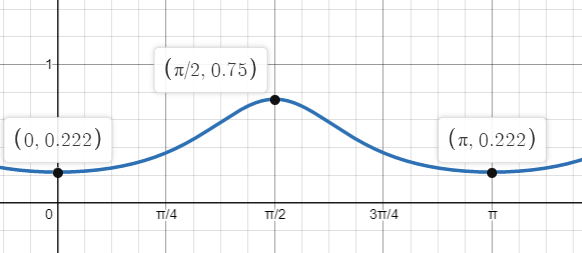
\includegraphics[width=0.3\textwidth]{3e.png}                                                                                                                                       \\
                  min                                         & = 0.222 \; max = 0.75                                                                                                                 \\
              \end{align*}
          \end{enumerate}
    \item Suppose a roller coaster path described by:
          $$\textbf{r}(t) = \frac{1}{5}t(20-t)\textbf{i} + \frac{1}{50}t^{2}(20-t)\textbf{j} + \frac{1}{50}t(10-t)(20-t)\textbf{k} \; : \; t \in [0,20]$$
          \begin{enumerate}
              \Item
              \begin{align*}
                  \textbf{v}(t) = \textbf{r}'(t) = \left(\frac{20-2t}{5}\right)\textbf{i} + \left(\frac{40t-3t^{2}}{50}\right)\textbf{j} + \left(\frac{3t^2-60t+200}{50}\right)\textbf{k} \\
              \end{align*}

              \Item
              \begin{align*}
                  \textbf{v}(5) & = 2 \textbf{i} + 2.5 \textbf{j} - 0.5 \textbf{k}                                         \\
                  \textit{v}    & = \left\| \textbf{v}(5) \right\| = \sqrt{2^2 + 2.5^2 + (-0.5)^2} = \sqrt{10.5} = 3.24037
              \end{align*}

              \Item
              \begin{align*}
                  \textbf{a}(t) = \textbf{v}'(t) = \textbf{r}''(t) = -\frac{2}{5}\textbf{i} + \left(\frac{40-6t}{50}\right)\textbf{j} + \left(\frac{6t-60}{50}\right)\textbf{k} \\
              \end{align*}

              \Item
              \begin{align*}
                  \kappa(t)                                         & = \frac{\| \textbf{v}(t) \times \textbf{a}(t) \|}{\| \textbf{v}(t) \|^3}                              \\
                  \textbf{v}(5)                                     & = 2 \textbf{i} + 2.5 \textbf{j} - 0.5 \textbf{k}                                                      \\
                  \| \textbf{v}(5) \|^3                             & = \left(\sqrt{10.5}\right)^3 = 34.023889                                                              \\
                  \textbf{a}(5)                                     & = -0.4 \textbf{i} + 0.2 \textbf{j} - 0.6 \textbf{k}                                                   \\\\
                  \textbf{v}(5) \times \textbf{a}(5)                & =
                  \begin{vmatrix}
                      \textbf{i} & \textbf{j} & \textbf{k} \\
                      2          & 2.5        & -0.5       \\
                      -0.4       & 0.2        & -0.6       \\
                  \end{vmatrix}                                                                                                                                \\
                                                                    & = (2.5(-0.6) - 0.2(-0.5))\textbf{i} - (2(-0.6)-(-0.4)(-0.5))\textbf{j} + (2(0.2)-2.5(-0.4))\textbf{k} \\
                                                                    & = -1.4\textbf{i} + 1.4\textbf{j} + 1.4\textbf{k}                                                      \\
                  \left\|\textbf{v}(5) \times \textbf{a}(5)\right\| & = \sqrt{(-1.4)^2 + 1.4^2 + 1.4^2} = \sqrt{5.88} = 2.424871                                            \\
                  \kappa(5)                                         & = \frac{\sqrt{5.88}}{\sqrt{10.5}^3} = 0.07127                                                         \\
              \end{align*}
              \Item\\
          \end{enumerate}
\end{enumerate}


\end{document}